\documentclass[12pt, letterpaper, twoside]{article}
\usepackage[utf8]{inputenc}
\usepackage[spanish]{babel}
\usepackage{amsmath, amsfonts, amssymb, amsthm}
\usepackage[left = 2cm, right = 2cm, top = 2cm, bottom = 2cm]{geometry}

\title{Material de referencia para la ICPC.}
\author{}
\date{} 

%Estilo de la página
\usepackage{fancybox, fancyhdr}
\pagestyle{fancy}
\fancyhf{}
\fancyhead[LE,RO]{\small{\leftmark}}
\fancyfoot[CE,CO]{\thepage}
\renewcommand{\headrulewidth}{2 pt}

%Imagenes
\usepackage{graphicx}

%Estilo del codigo
\usepackage{listings}
\usepackage[dvipsnames]{xcolor}
\lstset{  
	language         = C++, 
	xleftmargin      = 1 cm,
	numbers          = left,
	numberstyle      = \tiny\textbf,	
	basicstyle       = \footnotesize,
	keywordstyle     = \color{blue},
	directivestyle   = \color{Green},
	commentstyle     = \color{purple},
	stringstyle      = \color{blue},
	showstringspaces = false,
	breaklines       = true,
}

%Documento
\begin{document}

\maketitle

\tableofcontents

\newpage

\section{Estructuras de datos.}

\subsection{Policy Based Data Structures.}

La STL de GNU C++ implementa algunas estructuras de datos adicionales. Probablemente la más interesante de todas, es el árbol. Para poder utilizarlo debemos añadir antes las siguientes librerías:

\begin{lstlisting}
#include <ext/pb_ds/assoc_container.hpp>
#include <ext/pb_ds/tree_policy.hpp>
using namespace __gnu_pbds;
\end{lstlisting}

Los contenedores basados en árboles tienen la siguiente declaración:

\begin{lstlisting}
tree<Key, Mapped, Cmp_Fn = std::less<Key>, Tag = rb_tree_tag, node_update = null_node_update, Allocator = std::allocator<char> >
\end{lstlisting}

donde
\begin{itemize}
\item \texttt{Key} es el tipo de las llaves.

\item \texttt{Mapped} es el tipo de los datos mapeados. Esto se asemeja bastante a un \texttt{map}. Si en cambio lo llenamos con \texttt{null\_type}, obtenemos un contenedor similar a un \texttt{set}.

\item \texttt{Cmp\_Fn} es una función de comparación de llaves. Debe declararse en forma de \texttt{struct} con el operador \texttt{()} sobrecargado.

\item \texttt{Tag} especifica la estructura de datos a utilizar. Debe ser alguno de \texttt{rb\_tree\_tag} (red-black tree), \texttt{splay\_tree\_tag} (splay tree) o \texttt{ov\_tree\_tag} (ordered-vector tree).

\item \texttt{node\_update} especifica como actualizar los invariantes de cada nodo. El valor por defecto, \texttt{null\_node\_update}, indica que los nodos no guardan información adicional.
\end{itemize}

\textbf{Split y join}

Los contenedores basados en árboles soportan las mismas funciones que \texttt{set} y \texttt{map}, junto con dos funciones adicionales: 

\begin{lstlisting}
A.split(T key, Tree B);
A.join(Tree B);
\end{lstlisting}

La función \texttt{split} mueve todos los nodos con llaves mayores que \texttt{key} del árbol \texttt{A} al árbol \texttt{B}. La función \texttt{join}, por el contrario, mueve todos los nodos del árbol \texttt{B} al árbol \texttt{A}, siempre y cuando los rangos no se traslapen. En el caso de árboles rojo-negro, ambas funciones tienen complejidad poli-logarítmica.\medskip

\textbf{Iteradores de nodo}

Además de los iteradores convencionales de \texttt{set} y \texttt{map}, los contenedores basados en árboles implementan un tipo de iterador adicional, \texttt{node\_iterator}, el cual nos permite recorrer el árbol. Así por ejemplo, las funciones
\begin{lstlisting}
Tree::node_iterator root = A.node_begin();
Tree::node_iterator nil = A.node_end();
\end{lstlisting}
regresan un iterador de nodo correspondiente a la raíz y nodos nulos del árbol. Cada iterador de nodo incluye dos funciones miembro \texttt{get\_l\_child()} y \texttt{get\_r\_child()} que regresan los iteradores de nodos correspondientes a los hijos izquierdo y derecho.

Podemos hacer la conversión entre iteradores convencionales e iteradores de nodo de la siguiente manera:
\begin{lstlisting}
it = *nd_it;
nd_it = it.m_p_nd;
\end{lstlisting}
La primera línea regresa el \texttt{iterator} correspondiente a un \texttt{node\_iterator} mientras que la segunda realiza justamente lo contrario.\medskip

\textbf{Actualización de nodos}

Por otro lado, recordemos que \texttt{node\_update} especifica la información adicional que guardará cada nodo así como la forma en que se actualiza. Este debe ser declarado en forma de \texttt{struct}, el cual debe definir en su interior el tipo del dato adicional como \texttt{metadata\_type}, y sobrecargar el operador \texttt{()} especificando cómo se actualizará cada nodo. 

El operador \texttt{()} será llamado internamente cada vez que sea necesario, recibiendo como parámetros el nodo a actualizar y el nodo nulo. Las llamadas siempre se realizarán desde las hojas hasta la raíz. De esta manera, al actualizar la información de un nodo, se presupone que la información de sus hijos ya está actualizada.

Finalmente, cada iterador de nodo tiene una función miembro \texttt{get\_metadata()} que regresa una referencia al dato adicional de ese nodo. Sin embargo, al ser una variable constante, debemos hacerle antes un \texttt{const\_cast<metadata\_type \&>} para modificarlo.

Por ejemplo, si queremos que cada nodo guarde el tamaño del sub-árbol correspondiente, podemos definir la etiqueta \texttt{size\_node\_update} de la siguiente manera:

\begin{lstlisting}
template<typename node_const_iterator, typename node_iterator, typename Cmp_Fn, typename Allocator>
struct size_node_update {
    typedef int metadata_type;

    void operator() (node_iterator nd_it, node_const_iterator nil) {
        int lsize = 0, rsize = 0;
        if (nd_it.get_l_child() != nil)
            lsize = nd_it.get_l_child().get_metadata();
        if (nd_it.get_r_child() != nil)
            rsize = nd_it.get_r_child().get_metadata();
        const_cast<int &>(nd_it.get_metadata()) = lsize + rsize + 1;
    }
};
\end{lstlisting}

\textbf{Árbol de Estadísticos de Orden}

La STL incluye una etiqueta \texttt{tree\_order\_statistics\_node\_update}, que le indica a cada nodo que guarde el tamaño del sub-árbol correspondiente. Esta etiqueta incorpora dos funciones nuevas:
\begin{lstlisting}
A.find_by_order(unsigned int k);
A.order_of_key(T key);
\end{lstlisting}
La función \texttt{find\_by\_order} regresa un iterador convencional que corresponde al $k$-ésimo elemento de \texttt{A} (indexados en 0). La función \texttt{order\_of\_key}, por su parte, regresa un entero no negativo que representa el número de elementos menores que \texttt{key}. Ambas funciones tienen complejidad logarítmica.

\lstinputlisting[firstline = 6]{Estructuras/PolicyBased.cpp} \medskip

\newpage

\section{Grafos.}

\subsection{Caminos más cortos.}

\textbf{Algoritmo de Dijkstra.} Complejidad: $O((E + V) \log V)$.

\lstinputlisting[firstline = 6]{Grafos/Dijkstra.cpp}

\begin{tabular}{|p{7cm}|p{7cm}|}
\hline
\textbf{Entrada} & \textbf{Salida}\\ \hline
6 7    & 0: -1 0\\
0 1 4  & 1: 0 4\\
1 3 10 & 2: 0 2\\
3 5 11 & 3: 4 9\\
1 2 5  & 4: 2 5\\
2 0 2  & 5: 3 20\\
2 4 3  & \\
4 3 4  & \\
0      & \\ \hline
\end{tabular}

\begin{center}
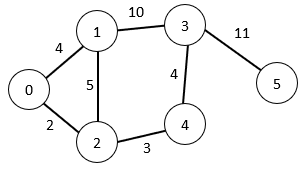
\includegraphics[width = 0.42\textwidth]{Grafos/Imagenes/ShortestPath.png}
\end{center}

\subsection{Árbol de expansión mínima.}

\textbf{Algoritmo de Kruskal.} Complejidad: $O(E \log V)$.

\lstinputlisting[firstline = 6]{Grafos/Kruskal.cpp}

\begin{tabular}{|p{7cm}|p{7cm}|}
\hline
\textbf{Entrada} & \textbf{Salida}\\ \hline
6 8    & Peso total: 18\\
0 1 2  & 0 3 1\\
0 3 1  & 3 5 1\\
3 1 9  & 0 1 2\\
4 1 10 & 3 4 3\\
3 4 3  & 2 0 11\\
2 0 11 & \\
2 5 20 & \\
3 5 1  & \\ \hline
\end{tabular}

\begin{center}
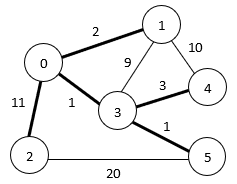
\includegraphics[width = 0.34\textwidth]{Grafos/Imagenes/MST.png}
\end{center}

\subsection{Orden topológico.}

Complejidad: $O(V + E)$.

\lstinputlisting[firstline = 6]{Grafos/TopoSort.cpp}

\begin{tabular}{|p{7cm}|p{7cm}|}
\hline
\textbf{Entrada} & \textbf{Salida}\\ \hline
7 9 & 6 0 1 2 5 4 3\\
6 1 & \\
6 5 & \\
0 1 & \\
1 5 & \\
0 2 & \\
1 2 & \\
2 3 & \\
5 3 & \\ 
5 4 & \\ \hline
\end{tabular}

\begin{center}
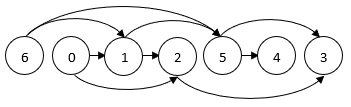
\includegraphics[width = 0.55\textwidth]{Grafos/Imagenes/TopoSort.png}
\end{center}

\subsection{Componentes fuertemente conexas.}

\textbf{Algoritmo de Tarjan.} Complejidad: $O(V + E)$.

\lstinputlisting[firstline = 6]{Grafos/Tarjan.cpp}

\begin{tabular}{|p{7cm}|p{7cm}|}
\hline
\textbf{Entrada} & \textbf{Salida}\\ \hline
6 8 & 4 5\\
0 1 & 2\\
1 2 & 3 1 0\\
1 4 & \\ 
1 3 & \\
3 0 & \\
2 5 & \\
4 5 & \\
5 4 & \\ \hline
\end{tabular}

\begin{center}
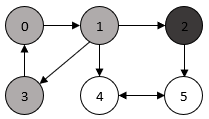
\includegraphics[width = 0.32\textwidth]{Grafos/Imagenes/StronglyConnected.png}
\end{center}

\subsection{Puentes y puntos de articulación.}

Complejidad: $O(V + E)$.

\lstinputlisting[firstline = 6]{Grafos/Bridge-Articulation.cpp}

\begin{tabular}{|p{7cm}|p{7cm}|}
\hline
\textbf{Entrada} & \textbf{Salida}\\ \hline
7 8 & Puntos de articulacion:\\
0 2 & 1 2 3\\
0 1 & Puentes:\\
1 2 & 1 6\\ 
1 6 & 2 3\\
2 3 & \\
3 4 & \\
4 5 & \\
3 5 & \\ \hline
\end{tabular}

\begin{center}
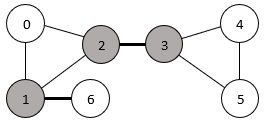
\includegraphics[width = 0.42\textwidth]{Grafos/Imagenes/Bridge-Articulation.png}
\end{center}

\subsection{Flujo máximo.}

\textbf{Algoritmo de Dinic.} Complejidad: $O(V^2 E)$.

\lstinputlisting[firstline = 6]{Grafos/Dinic.cpp}

\begin{tabular}{|p{7cm}|p{7cm}|}
\hline
\textbf{Entrada} & \textbf{Salida}\\ \hline
6 8    & Flujo maximo: 20\\
0 5    & 0 1: 11/11\\ 
0 1 11 & 0 2: 9/12\\
0 2 12 & 1 3: 12/12\\
1 3 12 & 2 1: 1/1\\
2 1 1  & 2 4: 8/10\\
2 4 10 & 3 5: 15/15\\
4 3 7  & 4 3: 3/7\\
3 5 15 & 4 5: 5/5\\
4 5 5  & \\ \hline
\end{tabular}

\begin{center}
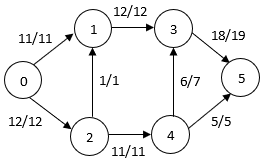
\includegraphics[width = 0.41\textwidth]{Grafos/Imagenes/MaxFlow.png}
\end{center}

\subsection{Emparejamiento máximo.}

\textbf{Algoritmo de Hopcroft-Karp.} Complejidad: $O(E \sqrt{V})$.

\lstinputlisting[firstline = 7]{Grafos/Hopcroft-Karp.cpp}

\begin{tabular}{|p{7cm}|p{7cm}|}
\hline
\textbf{Entrada} & \textbf{Salida}\\ \hline
5 4 8 & Emparejamiento: 3\\
1 1   & 1 - 1\\
2 1   & 2 - 3\\
2 3   & 3 - 2\\
3 2   & \\
3 3   & \\
3 4   & \\
4 3   & \\
5 3   & \\ \hline
\end{tabular}

\begin{center}
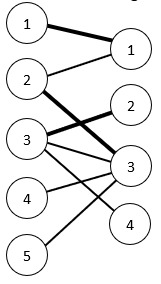
\includegraphics[height = 0.27\textheight]{Grafos/Imagenes/MaxMatching.png}	
\end{center}

\newpage

\section{Matemáticas.}

\subsection{Fórmulas importantes.}

\textbf{Desarreglos}

Un desarreglo es una permutación donde ningún elemento aparece en su posición original. El número de desarreglos está dado por la fórmula recursiva 
$$!n = (n - 1)(!(n - 1) + !(n - 2)), \qquad !0 = 1, \, !1 = 0$$ 
y por la fórmula cerrada
$$!n = n! \sum_{k=0}^n \frac{(-1)^k}{k!}.$$

\textbf{Números de Catalán}

Los números de Catalán cuentan: el número de expresiones con $n$ pares de paréntesis correctamente balanceados; el número de caminos distintos sobre una cuadrícula de $n \times n$ que empiezan en la esquina inferior izquierda y terminan en la esquina superior derecha, constan solamente de movimientos hacia arriba y hacia la derecha, y nunca cruzan la diagonal; el número de triangulaciones de un polígono convexo de $n + 2$ lados; entre otras cosas. Están dados por la fórmula recursiva
$$C_{n+1} = \sum_{i=0}^n C_iC_{n-i}, \qquad C_0 = 1$$
y por la fórmula cerrada
$$C_n = \frac{1}{n + 1}\binom{2n}{n}.$$

\textbf{Números de Stirling}

Los números de Stirling de primer tipo cuentan el número de permutaciones con exactamente $k$ ciclos disjuntos. Están dados por la fórmula recursiva
$$c(n + 1, k) = nc(n, k) + c(n, k - 1), \qquad c(n, 0) =  0, \, c(n, n) = 1.$$

Los números de Stirling de segundo tipo cuentan el número de particiones de un conjunto de tamaño $n$ en $k$ subconjuntos no vacíos. Están dados por la fórmula recursiva
$$S(n + 1, k) = kS(n, k) + S(n, k - 1), \qquad S(n, 0) =  0, \, S(n, n) = 1$$
y por la fórmula cerrada
$$S(n, k) = \frac{1}{k!} \sum_{i=0}^k (-1)^i \binom{k}{i}(k - i)^n.$$

\textbf{Números de Grundy}

Un juego por turnos entre dos jugadores es \textit{normal} si el jugador que no pueda mover pierde, y es \textit{imparcial} si en todo momento ambos jugadores disponen del mismo conjunto de movimientos.

El juego de \textit{Nim} es un juego normal e imparcial en donde cada jugador debe escoger una pila y eliminar al menos un objeto de esa pila. Sean $P_1, \ldots, P_n$ los tamaños de cada pila. El jugador en turno tiene estrategia ganadora si y sólo si $P_1 \text{ xor } \ldots \text{ xor } P_n \neq 0$.

El \textbf{Teorema de Sprague-Grundy} afirma que todo juego normal e imparcial es equivalente a un juego de Nim.

\subsection{Big Numbers.}

\lstinputlisting[firstline = 6]{Matematicas/BigNumbers.cpp}

\begin{tabular}{|p{7cm}|p{7cm}|}
\hline
\textbf{Entrada} & \textbf{Salida}\\ \hline
1894821 & 1894821 + 589613 = 2484434\\
589613  & 1894821 - 589613 = 1305208\\ 
& 1894821 * 589613 = 1117211094273\\ 
& 1894821 = 589613 * 3 + 125982\\ \hline
\end{tabular}\bigskip

\subsection{Test de Primalidad.}

\textbf{Algoritmo de Miller-Rabin.}

\lstinputlisting[firstline = 6]{Matematicas/Miller-Rabin.cpp} 

\begin{tabular}{|p{7cm}|p{7cm}|}
\hline
\textbf{Entrada} & \textbf{Salida}\\ \hline
1000000007 & Probablemente es primo.\\
123456789  & No es primo.\\
104729     & Probablemente es primo.\\ \hline
\end{tabular}\bigskip

\subsection{Factorización en primos.}

\textbf{Algoritmo de prueba por división.} Complejidad: $O\left(\pi\left(\sqrt{n}\right)\right)$ donde $\pi(x)$ es el número de primos menores o iguales que $x$.

\lstinputlisting[firstline = 6]{Matematicas/Trial-Division.cpp}

\begin{tabular}{|p{7cm}|p{7cm}|}
\hline
\textbf{Entrada} & \textbf{Salida}\\ \hline
180   & 2 2 3 3 5\\
3500  & 2 2 5 5 5 7\\ 
123456789 & 3 3 3607 3803\\
104729 & 104729\\ \hline
\end{tabular}\bigskip

\subsection{Sistemas de Ecuaciones Lineales.}

\textbf{Eliminación Gaussiana.} Complejidad $O(n^3)$.

\lstinputlisting[firstline = 6]{Matematicas/GaussianElimination.cpp}

\begin{tabular}{|p{7cm}|p{7cm}|}
\hline
\textbf{Entrada} & \textbf{Salida}\\ \hline
4 1          & Determinante: 142\\
1 -2 2 -3 15 & Solucion:\\ 
3 4 -1 1 -6  & 2\\ 
2 -3 2 -1 17 & -2\\ 
1 1 -3 -2 -7 & 3\\ 
             & -1\\ \hline
\end{tabular}\bigskip

\subsection{Teorema Chino del Residuo.}

\lstinputlisting[firstline = 6]{Matematicas/ChineseRemainder.cpp}

\begin{tabular}{|p{7cm}|p{7cm}|}
\hline
\textbf{Entrada} & \textbf{Salida}\\ \hline
3   & x = 66 (mod 180)\\
2 4 & \\ 
3 9 & \\ 
1 5 & \\ \hline
\end{tabular}

\newpage

\section{Strings}

\subsection{Búsqueda de patrones.}

\textbf{Arreglo Z.} Complejidad: $O(|P| + |T|)$.

\lstinputlisting[firstline = 6]{Strings/Z-Array.cpp}

\begin{tabular}{|p{7cm}|p{7cm}|}
\hline
\textbf{Entrada} & \textbf{Salida}\\ \hline
AABAACAADAABAABA & Patron encontrado en la posicion 0\\
AABA             & Patron encontrado en la posicion 9\\
& Patron encontrado en la posicion 12\\ \hline
\end{tabular}\bigskip

\textbf{Aho Corasick.} Complejidad: $O(|T| + |P_1| + \ldots + |P_n| + \#Ocurrencias)$.

\lstinputlisting[firstline = 7]{Strings/Aho-Corasick.cpp}

\begin{tabular}{|p{7cm}|p{7cm}|}
\hline
\textbf{Entrada} & \textbf{Salida}\\ \hline
abcdabccabbacefdabc & abc aparece en la posicion 0\\
4                   & bcd aparece en la posicion 1\\
abc                 & abc aparece en la posicion 4\\
ca                  & ca aparece en la posicion 7\\
bcd                 & ef aparece en la posicion 13\\
ef                  & abc aparece en la posicion 16\\ \hline
\end{tabular}\bigskip

\subsection{Arreglo de sufijos.}

Complejidad: $O(|s|\log |s|)$.

\lstinputlisting[firstline = 6]{Strings/Suffix-Array.cpp}

\begin{tabular}{|p{7cm}|p{7cm}|}
\hline
\textbf{Entrada} & \textbf{Salida}\\ \hline
banana & 5 a\\
& 3 ana\\
& 1 anana\\
& 0 banana\\
& 4 na\\
& 2 nana\\ \hline
\end{tabular}

\newpage

\end{document}